\documentclass[../../main.tex]{subfiles}

\begin{document}
\graphicspath{{imgs/}{02_theory/imgs/}}

% \chapterimage{chapter_head_1.pdf}
\chapter{Position Estimation}

\section{Signal parameters}

There are two approaches for positioning: direct and two-step. In the direct approach, the signal is used for positioning itself. In the two-step approach, positioning is base on parameters extracted from the signal but not the signal itself. One consideration is that in two-step approach, parameters may be extracted from a similar but undesired signal; in the direct approach, it is possible to verify the signal's origin. The two-step approach imposes less complexity and is close in performance to the direct approach, os the two-step approach is more prevalent in practice and is the focus of this report.

\begin{figure}[h]
    \centering
    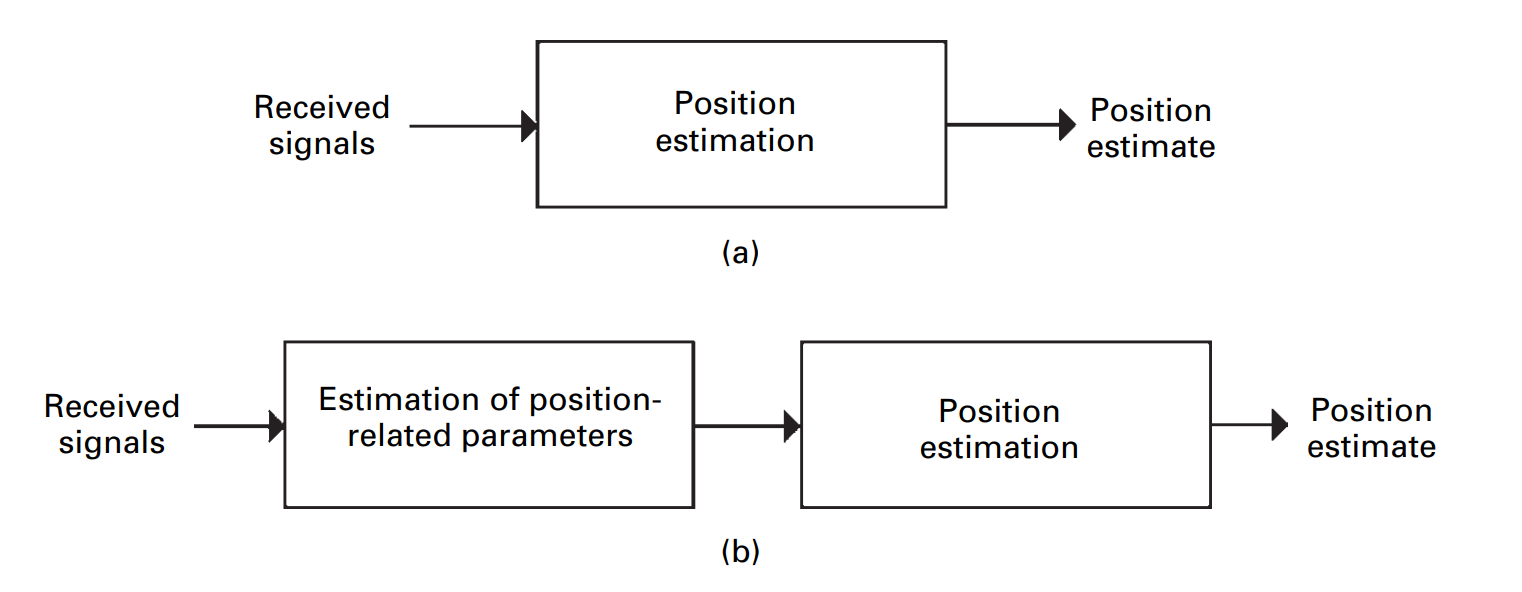
\includegraphics[width=0.8\textwidth]{direct_positioning_vs_two_step_positioning}
    \caption{(a) Direct positioning, (b) Two-step positioning}
    \label{fig:direct_positioning_vs_two_step_positioning}
\end{figure}

\subsection{Received Signal Strength}
The strength of a received signal is decreased by path loss (PL) which is proportional to the distance between transmitter ana receiver. So we can estimate the range to target node by measuring RSS. Ideally, the RSS matches $\overline{P}(d)$ in the following: 
\begin{equation}
    \overline{P}(d) = P\textsubscript{0}-10n\log_{10} \frac{d}{d\textsubscript{0}} 
\end{equation}
where:
\begin{itemize}
    \item $n$ is passloss exponent
    \item $\overline{P}(d)$ is the received power at distance $d$
    \item $P\textsubscript{0}$ is the received signal at the reference distance 
\end{itemize}

There are phenomena which affect the amount of PL. This first one is the multipath phenomena. Simply, it means that several components of one signal have followed some different paths to the receiver, experiencing different amounts of PL. We can overcome this problem by choosing a long enough interval for the following integration: 
\begin{equation}
    P(d) = \frac{1}{T} \int_0^T \left| r(t) \right| ^2 dt
\end{equation}
where $P(d)$ is the received power and $r(t)$ is the received signal.

The second phenomenon is shadowing or large-scale fading. The main reason for this phenomenon is a changing environment over a long-distance propagation. The effect of shadowing is modeled with a log-normal random variable:

\begin{equation}
    \label{eq:received_signal_model}
    10\log_{10} P(d) \sim \mathcal{N}(\overline{P}(d), \sigma_{sh}^2)\
\end{equation}
where $\overline{P}(d)$ is the average received power and $\sigma_{sh}^2$ is the variance of a Gaussian random variable $\mathcal{N}$.

For this model \ref{eq:received_signal_model}, the Cramer-Rao lower bound (CRLB) for estimating distance can be expessed as:
\begin{equation}
    \sqrt{Var\{\hat{d}\}} \geq \frac{\ln{10}}{10} \frac{\sigma_{sh}}{n} d
\end{equation}

where $\hat{d}$ is an unbiased estimate of $d$. We observe that the bigger the PL exponent $n$ is, the smaller the lower bound is. In additional, a smaller distance $d$ and smaller $\sigma_{sh}$ gives a smaller lower bound.

In figure \ref{fig:limits_for_distance_estimation_based_on_rss_measurements}, the mininmum standard devariation $\sigma_{\hat{d}}=\sqrt{Var\{\hat{d}\}}$ of several channels are plotted. The PL exponents and the standard deviations of the shadowing are given in Table \ref{table:channel_parameters_for_the_environments}.

\begin{table}[htbp]
    \begin{tabularx}{1\textwidth} { 
         >{\raggedright\arraybackslash}X 
         >{\centering\arraybackslash}X 
         >{\centering\arraybackslash}X }
            \hline \hline
            & n & $\sigma_{sh}$  \\ 
            \hline
            Residential LOS & 1.79 & 2.22  \\ 
            \hline
            Residential NLOS & 4.58 & 3.51 \\
            \hline
            Indoor office LOS & 1.63 & 1.90 \\
            \hline
            Indoor office NLOS & 3.07 & 3.90 \\
            \hline \hline
      \end{tabularx}
      \caption{Channel parameters for the environments}
      \label{table:channel_parameters_for_the_environments}
\end{table}

\begin{figure}[htbp]
    \centering
    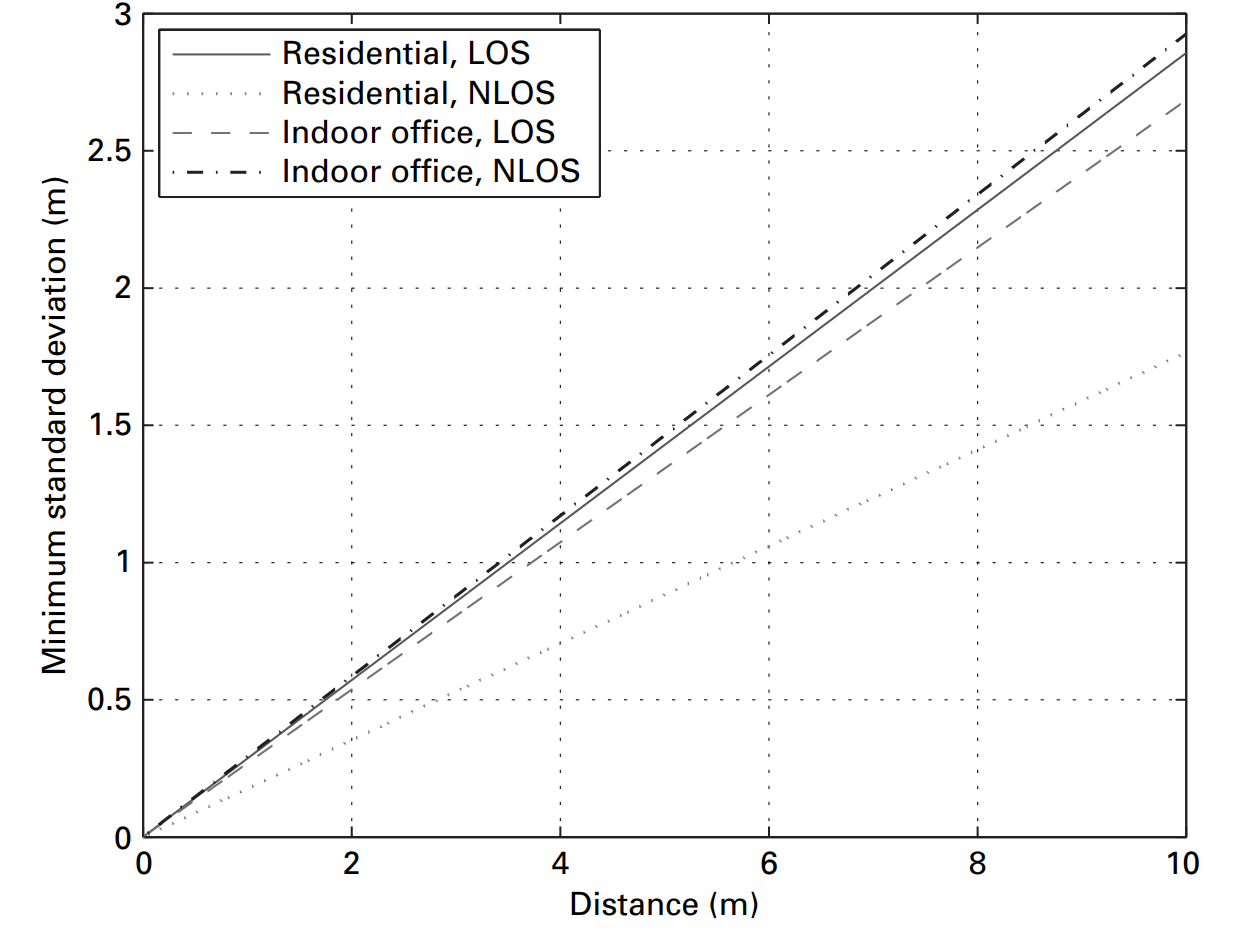
\includegraphics[width=0.8\textwidth]{limits_for_distance_estimation_based_on_rss_measurements}
    \caption{Theoretical limits for distance estimation based on RSS measurements at different distances for various channel models}
    \label{fig:limits_for_distance_estimation_based_on_rss_measurements}
\end{figure}

\subsection{Time of arrival (TOA)}

The time of arrival (TOA) method gives us information about the distance between the target node and the source for which the position is known. The target node's position is on a circle of radius $d=c\tau$, for $c$ equal speed of light and $\tau$ equal time of arrival. The prerequisite of this information is a synchronization between the source and target node. The received signal at the source node is represented by:
\begin{equation}
    r(t) = \alpha(t-\tau) + n(t)
\end{equation}
where $\tau$ is the TOA, $\alpha$ is the channel coefficient and $n(t)$ is white Gaussian noise with zero mean and a spectral density of $\mathcal{N}_0/2$ watts per hertz for $\mathcal{N}$ is normal distribution. In order to extract TOA from received signal, we search for the maximum correlation between the shifted version of template signal ($s(t-\hat{\tau})$) and the received signal. The $\hat{\tau}$ which gives the peek correlation provides an estimation of the TOA. For signal model \ref{eq:received_signal_model} , the CRLB is:
\begin{equation}
    \sqrt{Var\{\hat{\tau}\}} \geq \frac{1}{2\sqrt{2}\pi\sqrt{SNR}\beta}
\end{equation}
where $\tau$ is the estimation of TOA, $SNR = \alpha^2 E / \mathcal{N}_0$ is the signal to noise ratio, $\beta$ is the effective signal bandwidth and $E$ is the signal energy. One important property of TOA is that, unlike RSS, its accuracy heavily depend on the bandwidth of the signal. Consequently, UWB systems can reach very precise ranging on he order of a few centimeters. Figure \ref{fig:toa_minimum_standard_deviation_versus_bw_snr} shows the effects of $SNR$ and band width on the accuracy of TOA estimation.

\begin{figure}[htbp]
    \centering
    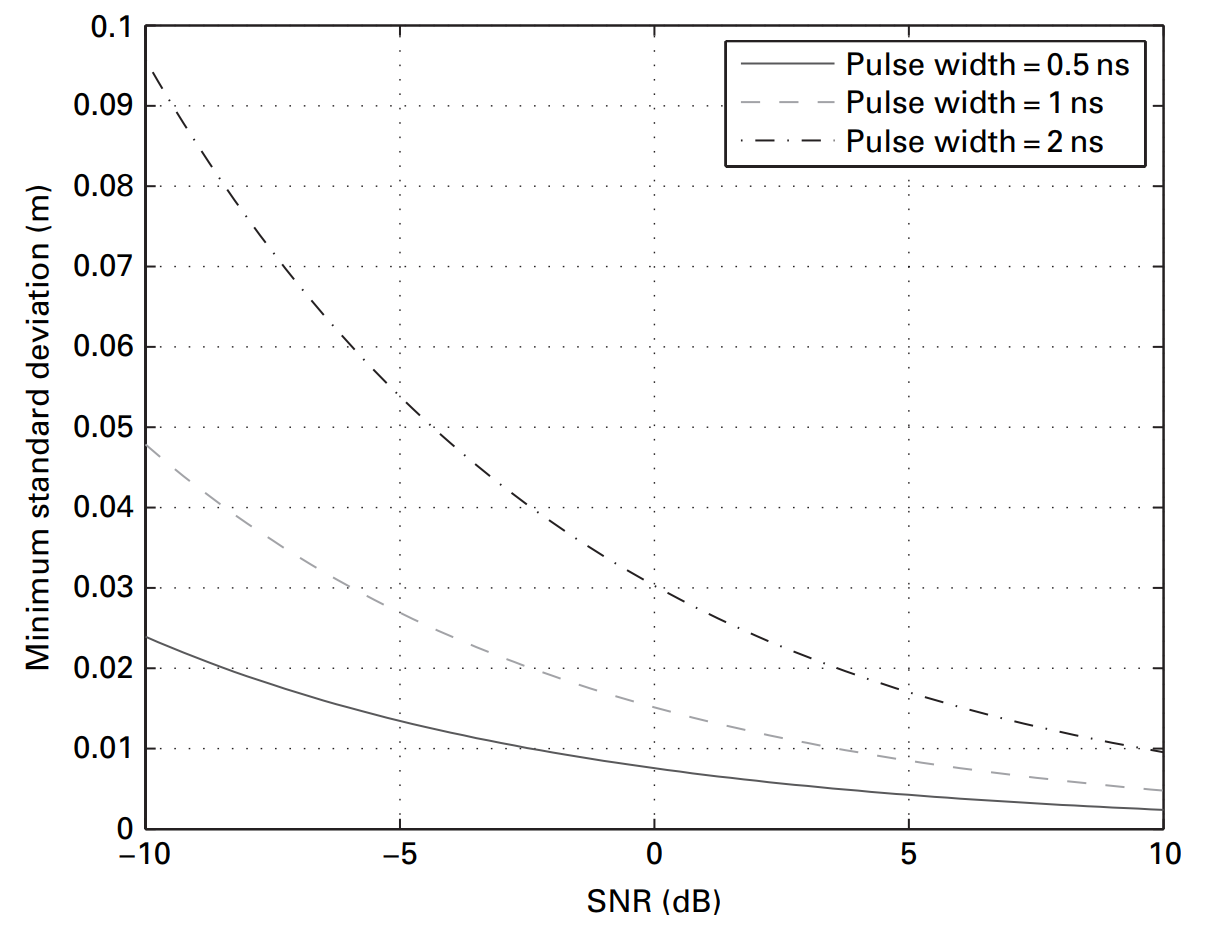
\includegraphics[width=0.8\textwidth]{toa_minimum_standard_deviation_versus_bw_snr}
    \caption{The minimum standard deviation versus SNR for various pulse widths}
    \label{fig:toa_minimum_standard_deviation_versus_bw_snr}
\end{figure}

\subsection{Time difference of arrival (TDOA)}

In this approach, the extracted parameter is the difference between the arrival time of the transmitted signal (from the target node) to two source nodes. This parameter, by multiplying TDOA by the speed of light, gives us an uncertainty of the target node's position in the shape of a hyperbola as shown:

\begin{figure}[htbp]
    \centering
    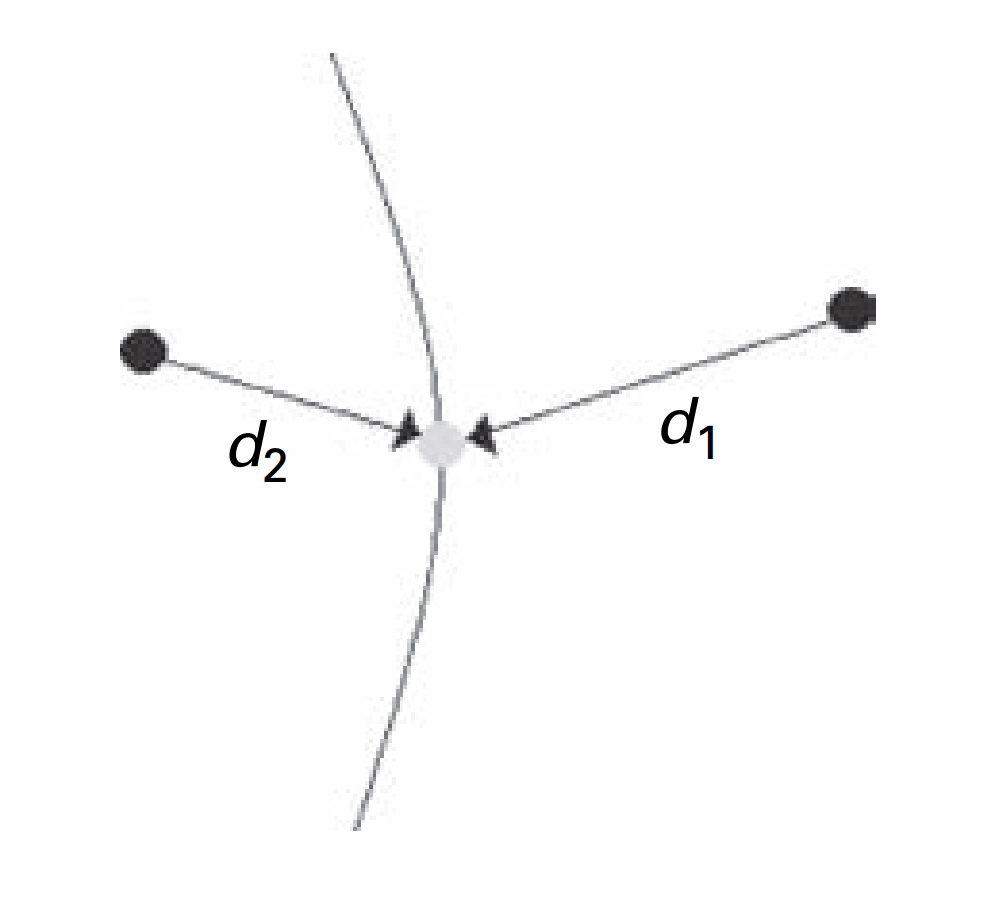
\includegraphics[width=0.5\textwidth]{tdoa_hyperbola}
    \caption{A TDOA measurement defines a hyperbola passing through the target node (gray node) with foci at the reference nodes (black nodes) }
    \label{fig:tdoa_hyperbola}
\end{figure}

The merit of TDOA in comparison with TOA is that there is no need for synchronization between source nodes and target nodes. Source nodes, however, do need to be synchronized. In the TOA base approach for measuring TDOA, TOA is measured at two source nodes which we call $\tau_1$ and $\tau_2$. As the source node and target node are not synchronized, there is a time offset in $\tau_1$ and $\tau_2$. Since the source are synchronized with themselves, this offset is equal in both measurements. Consequently, we can measure the TDOA as:
\begin{equation}
    \tau_{TDOA} = \tau_1 - \tau_2
\end{equation}
where $\tau_{TDOA}$ is the estimation of TDOA. In this approach, there is the same effect of bandwidth as in TOA measurements.
The second approach to measure the TDOA is using cross-correlation between two received signals. We know that there is some amount of offset between received signals so cross-correlation will reach maximum when one of the signals if shifted with correct offset. The cross-correlation equation is:
\begin{equation}
    \phi_{1,2}(\tau) = \frac{1}{T}\int_0^T r_1(t)r_2(t+\tau)dt
\end{equation}
where $r_1(t)$ and $r_2(t)$ are the received signals and $T$ is the observation interval. Then TDOA is estimated by:
\begin{equation}
    \tau_{TDOA}= \argmax_\tau \left| \phi_{1,2}(\tau) \right|
\end{equation}
where 
\begin{equation}
    \argmax_x f(x) := \{x | \forall y: f(y) \leq f(x)\}
\end{equation}
The correlation approach work well for white noise and single path channels but in the case of multi-path channel or colored noise, its performance decrease significantly.

\subsection{Angle of arrival (AOA)}

AOA is another parameter of the signal which includes include information about position target node. In this case, we estimate the angle, $\psi$, between an array of antennas and the target node regards to the delay between arrival of the signal to the antenna. AOA fives us an uncertainty region with the shape of a line, as depicted in figure \ref{fig:aoa_uncertainty_region}.

\begin{figure}[htbp]
    \centering
    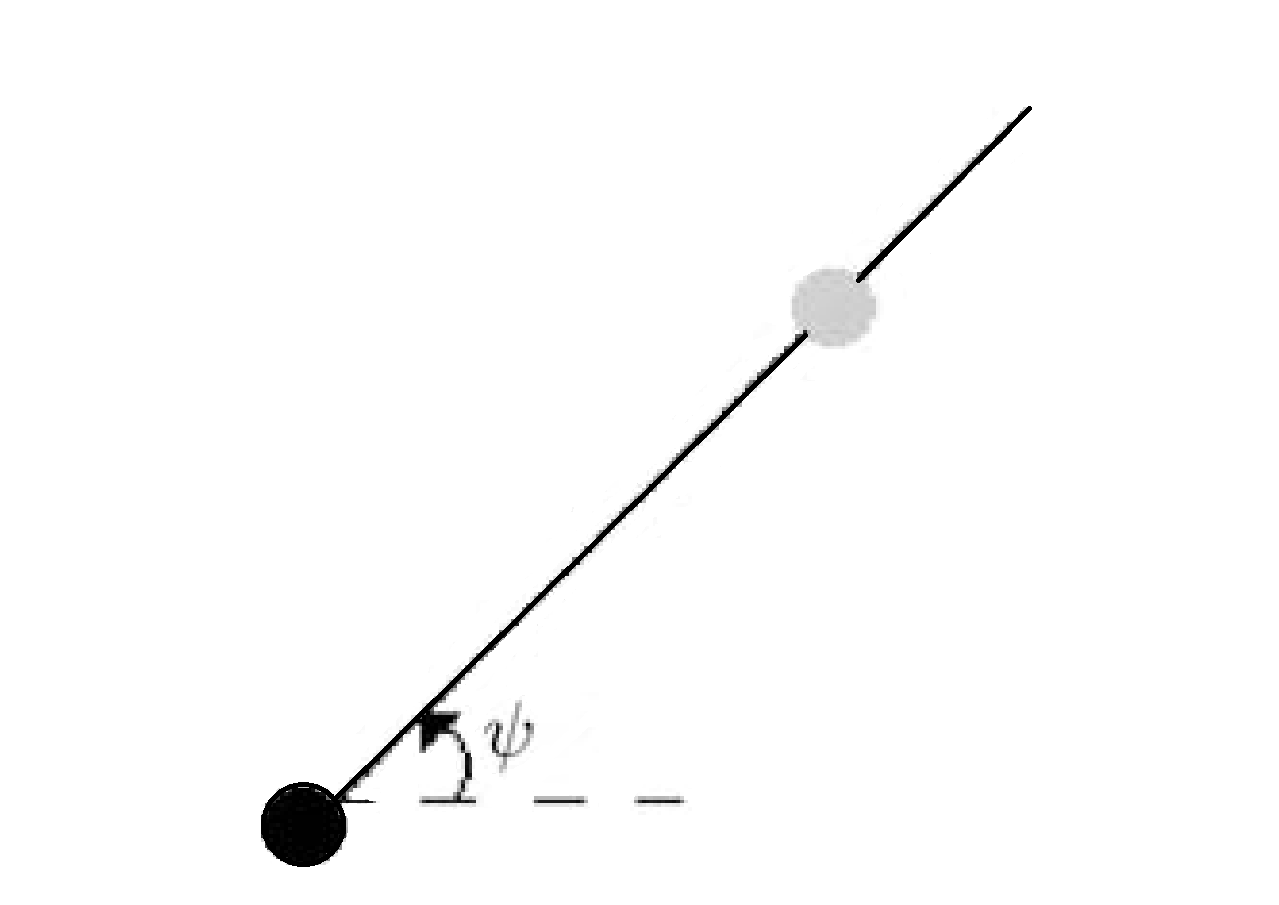
\includegraphics[width=0.3\textwidth]{aoa_uncertainty_region}
    \caption{The reference node (black node) measures the AOA and determines the angle $\psi$ between itself and the target node (gray node)  }
    \label{fig:aoa_uncertainty_region}
\end{figure}

The antenna array may be in different arrangements, the simplest one is the uniform linear array (ULA) as shown in figure \ref{fig:aoa_signal_arrival_at_a_ula}. In case of ULA, the delay between the arrival of the signals to the consecutive antenna is given by:
\begin{equation}
    \tau = \frac{l\sin{\psi}}{c}
\end{equation}

where $\tau$ is the delay, $l$ is the distance between consequent antennas, $\psi$ is the AOA and $c$ is the speed of light.

\begin{figure}[htbp]
    \centering
    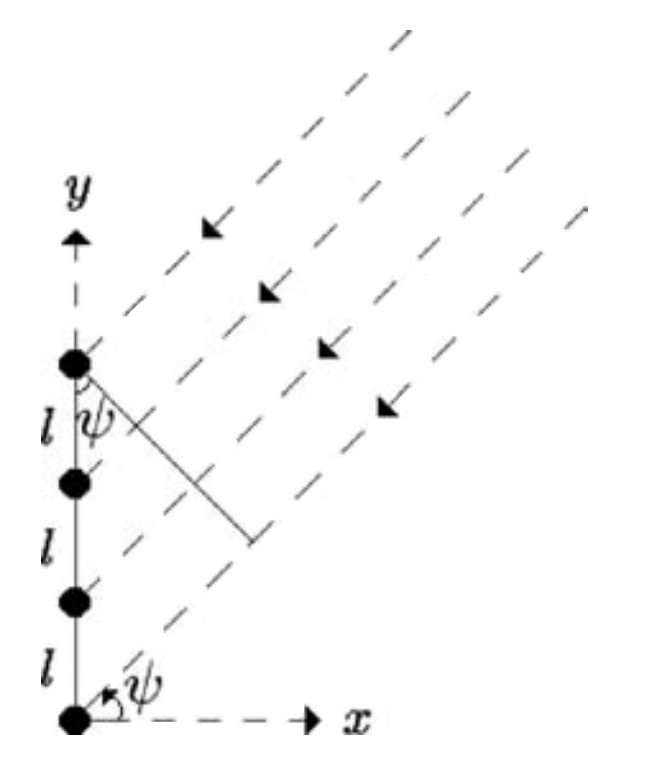
\includegraphics[width=0.3\textwidth]{aoa_signal_arrival_at_a_ula}
    \caption{Signal arrival at a ULA, and relation between arrival time differences and AOA}
    \label{fig:aoa_signal_arrival_at_a_ula}
\end{figure}

In order to measure the accuracy if the AOA approach, we formulate the received signal to each $N_a$ antennas by:

\begin{equation}
    r_i(t) = \alpha s(t-\tau_i) + n_i(t)
\end{equation}

where $\alpha$ is the coefficient of the channel, $\tau_i$ is the delay for the $i$th antenna and $n_i(t)$ is the white Gaussian noise with zero mean and spectral density of $\mathcal{N}_0/2$. We can express the delay of the signal received by the $i$th antenna as:
\begin{equation}
    \tau_i \approx \frac{d}{c} + \frac{l_i \sin{\psi}}{c}
\end{equation}
where
\begin{equation}
    l_i = l \left( \frac{N_a+1}{2} - i \right)
\end{equation}
and $d$ is the distance between the target node and the center of the antenna array. The CRLB for estimating $\psi$ is:
\begin{equation}
    \sqrt{Var\{\hat{\psi}\}} \geq \frac{\sqrt{3}c}{\sqrt{2}\pi\sqrt{SNR}\beta\sqrt{N_a(N_a^2-1)}l\cos{\psi}}
\end{equation}
We observe that the accuracy of the AOA method is dependent on $SNR$, $\beta$, $N_a$, $l$ and $\psi$. Our main interest is the effect of bandwidth on the accuracy since we use signals width very small pulse in time in the UWB systems. Figure \ref{fig:aoa_crlb_ for_angle_of_arrival_versus_snr} depicts the effect of the pulse width and SNR on CRLB for angle of arrival. In this case, other parameters are assume to be fixed.

\begin{figure}[!htbp]
    \centering
    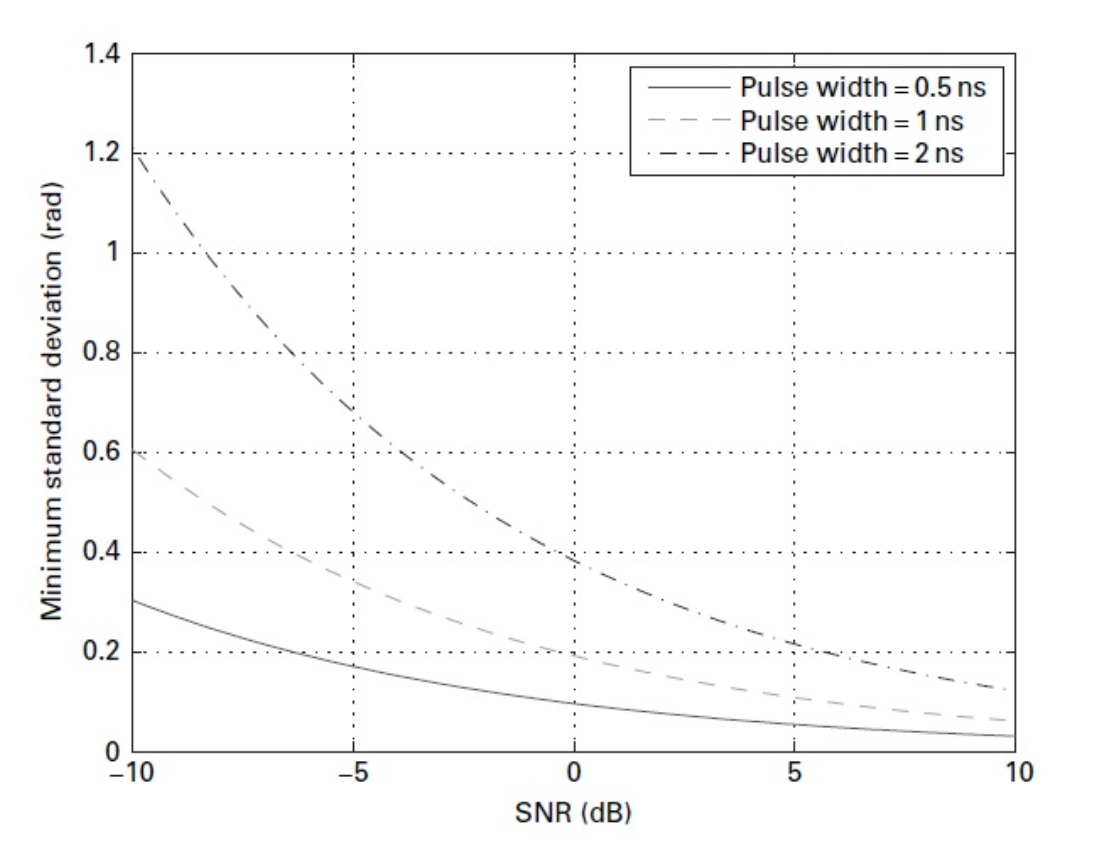
\includegraphics[width=0.8\textwidth]{aoa_crlb_for_angle_of_arrival_versus_snr}
    \caption{CRLB for the angle of arrival versus SNR for several pulse-widths}
    \label{fig:aoa_crlb_ for_angle_of_arrival_versus_snr}
\end{figure}
We observe that increasing bandwidth (decreasing pulse-width) has a significant effect on the accuracy. In other words, with high bandwidth, we can gain high accuracy even with low SNR. Consequently, UWB is a very good candidate for the AOA approach.

In figure \ref{fig:aoa_crlb_versus_psi_for_various_pulse_widths}, the effect of AOA on its estimation accuracy is depicted. We observe that even for wide-band signals, the accuracy will be decrease dramatically for angles bigger than 1 rad (57 degrees) or smaller than 1 rad. As a suggestion, we can use several antenna arrays and weight the estimation of each array by the inverse of estimated angle.
\begin{figure}[!htbp]
    \centering
    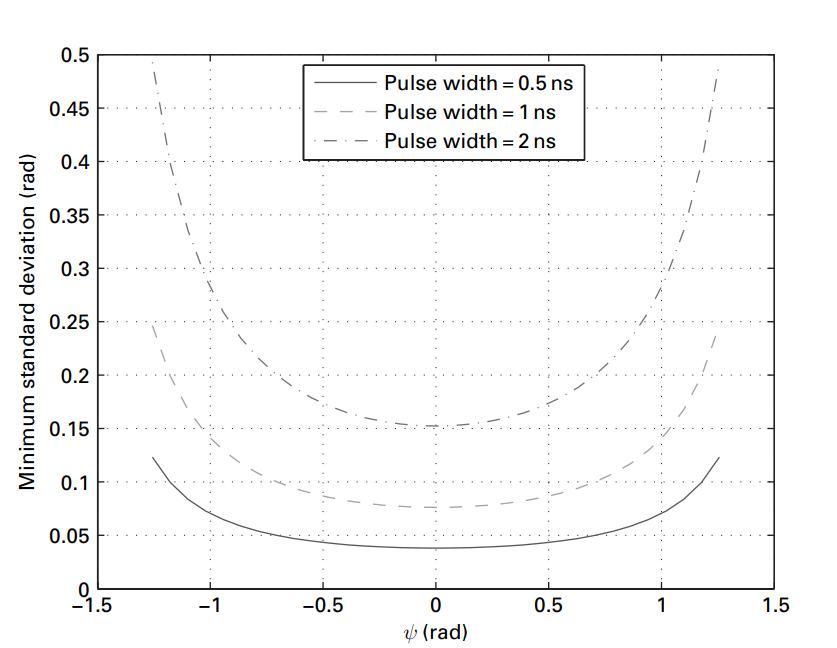
\includegraphics[width=0.8\textwidth]{aoa_crlb_versus_psi_for_various_pulse_widths}
    \caption{CRLB for the angle of arrival versus SNR for several pulse-widths}
    \label{fig:aoa_crlb_versus_psi_for_various_pulse_widths}
\end{figure}

\end{document}